\section{Introducción}

En el presente trabajo se realiza una amplia experimentación con la capa tres del modelo OSI, es decir, con el nivel de red. A partir de un desarrollo propio de la herramienta $traceroute$ (en su versión sobre mensajes ICMP) sobre el framework Scapy para python, se colectan muestras a lo largo del día de $round-trip time$ a 3 Universidades del mundo, así como también se colectan muestras utilizando otra implementación incluida en Linux de la misma aplicación. Debido a la variabilidad de esta medición, cada experimento se repite $n$ veces para luego obtener un promedio representativo de la colección de datos. En base a la implementación de traceroute en Python, se implementa además una heurística para poder identificar enlaces transatlánticos en la ruta, lo cual es objeto de la segunda parte de experimentación de este trabajo.\\

\begin{figure}[h!]
  \centering
  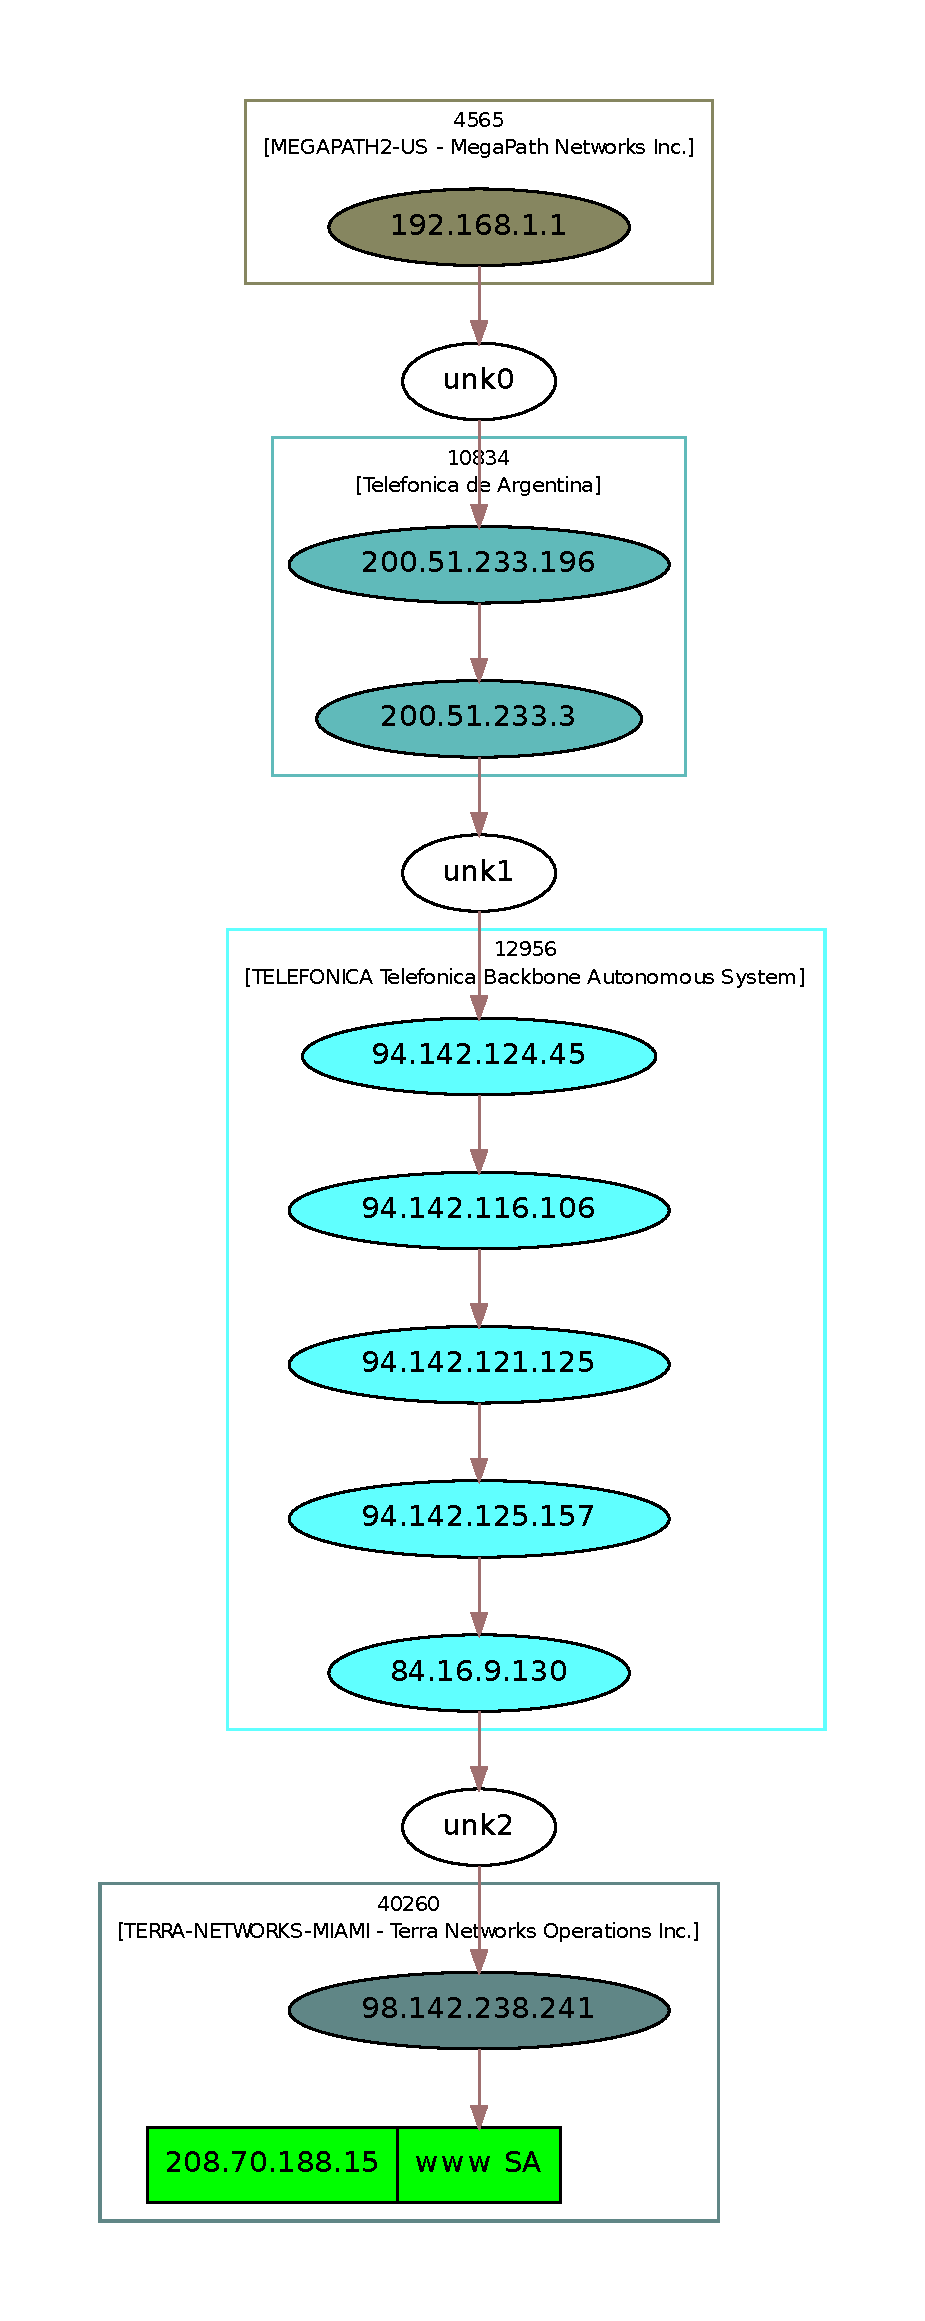
\includegraphics[width=0.4\textwidth]{./figs/ruta_google.pdf}
  \caption{Diagrama de una ruta trazada por $traceroute$ de Scapy}
\end{figure}
